\chapter{Simulations with the \pkg{specsim} package}

Introduction: used to generate simulations for eBOSS Lyman-alpha and to verify DESI sky model. 

\section{Spectroscopic simulations with \pkg{specsim}}

\pkg{specsim} (cite) is a software package developed by Dr. David Kirkby to simulate the response of a multi-fiber spectrograph. Although it was originally created to generate realistic synthetic spectra for the DESI instrument, it can be reconfigured to simulate any fiber-fed spectrograph, provided that the accompanying instrument parameter specifications and data are provided.\\

A single simulation consists of three components: a source spectrum, a model of the sky and atmosphere, and a model of the instrument. A schema of where each component comes into play is shown in Fig. \ref{fig:schema}, which shows the journey of photons as they are emitted from a galaxy to the moment they are read out by the detector.\\

\begin{figure}
\centering
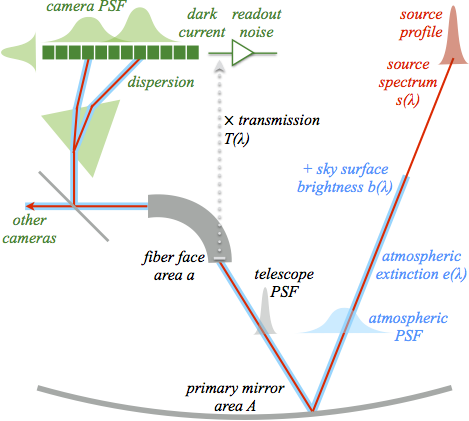
\includegraphics[width=11cm]{images/specsim/overview.png}
\caption{Specsim schema.}
\label{fig:schema}
\end{figure}

\subsection{Astrophysical source}
% Needs work/editing
Spectra of astrophysical sources are simulated individually, beginning with a spectral energy distribution (SED) in its rest frame, $s(\lambda)$, and its morphological profile. Configuration parameters for a source profile include the bulge/disk fraction and shape parameters such as the half-light radius, position angle, and the ratio of the semi-minor to semi-major axis. The source profile is assumed to be independent of its SED, and will come into play later on when accounting for fiberloss when modeling the effects of the instrument.\\ 

\begin{table}
\caption{Specsim simulation parameters.}
\label{tab:specsim_vars}
\centering
\begin{tabular}{|c|c|c|}
  \hline
  Parameter & Component & Description \\
  \hline \hline
  $\Delta t$ & Instrument & Exposure time \\
  \hline
  $X$ & Atmosphere & Observing airmass \\
  \hline
  $\lambda_{i}$ & Configuration & Fine wavelength grid \\
  \hline
  $s(\lambda)$ & Source & Source SED \\
  \hline
  $b(\lambda)$ & Atmosphere & Sky surface brightness \\
  \hline
  $e(\lambda)$ & Atmosphere & Atmospheric extinction \\
  \hline
  $A$ & Instrument & Primary unobscured area \\
  \hline
  $a$ & Instrument & Fiber entrance area \\
  \hline
  $f_{S}(\lambda)$ & Source \& Instrument & Fiberloss fraction \\
  \hline 
  $T_{i}(\lambda)$ & Camera & Transmission throughput \\
  \hline
  $d_{i}(\lambda)$ & Camera & CCD row width \\
  \hline
  \sigma_{i}(\lambda) & Camera & CCD resolution \\
  \hline
  $n_{ip}$ & Camera & CCD trace width \\
  \hline
  $I_{dk,i}$ & Camera & Sensor dark current \\
  \hline
  $G_{i}$ & Camera & CCD gain \\
  \hline
  $\sigma_{ro,i}$ & Camera & Readout noise \\
  \hline
\end{tabular}
\end{table}\\

\subsection{Sky model}
Given a source, the next component of the \pkg{specsim} pipeline is the sky model, which incorporates the effects of the atmosphere. The three elements that make up the sky model are a sky emission spectrum, the atmospheric point spread function, or PSF, and atmospheric extinction.\\

% Include side-by-side plots of DESI vs eBOSS dark sky here
% Talk about downsampling?

% Sky emission
The sky model used for both DESI and eBOSS configurations is virtually identical. The sky emission surface brightness $b(\lambda)$ for the DESI configuration contains data for three different types of sky spectra corresponding to dark, bright and grey conditions, whereas the eBOSS sky emmission spectrum is just the DESI dark sky extrapolated to cover the wider wavelength range of the eBOSS spectrograph.\\

% Seeing
Atmospheric PSF results in the blurring of an image of a source as its photons encounter varying indices of refraction when traveling through different layers of the Earth's atmosphere. Differences in temperature, pressure, density and molecular composition in each layer, as well as turbulence in the air, cause photons to slightly deflect from their original paths, resulting in a ``smeared" image. Seeing is defined as the full width at half maximum (FWHM) of a radial profile of a point source, typically a star, from its peak value.\\

The effects of atmospheric seeing in \pkg{specsim} can be applied in one of three ways. The fastest mode assumes a fixed 1.1" seeing for each source type (LRG, ELG, QSO, etc.), and doesn't account for any additional information about surface brightness profiles. A slower, but more flexible mode uses \pkg{GalSim}, a package that simulates images of astrophysical sources (cite), to convolve the source profile with the atmospheric PSF. \pkg{GalSim} requires additional information in the configuration file such as FWHM$_{ref}$ and $\lambda_{ref}$, which are used to estimate the PSF as a function of wavelength in the following way:

\begin{equation}
    \mbox{FWHM}(\lambda) = \mbox{FWHM}_{ref} \Big(\frac{\lambda}{\lambda_{ref}}\Big)^{-0.2}.
\end{equation}

Since \pkg{GalSim} uses a Moffat profile to model the PSF, a fixed value for the $\beta$ parameter, which determines the shape of the PSF, must also be specified. The Moffat distribution is predominantly used for modeling PSFs as it is more successful at capturing tails compared to a Gaussian or Lorentzian distribution.

The final component in the sky model is atmospheric extinction, which could be caused by Rayleigh scattering of air molecules or particulate matter such as aerosols, or by telluric absorption due to the Earth's atmosphere. This is provided in the configuration file as a list of tabulated values for the extinction coefficient $e(\lambda)$ at zenith as a function of wavelength. The amount of extinction at other airmasses is determined by multiplying the the extinction coefficient by the airmass at that particular pointing.\\

Together, the three components of the sky model can be combined to model the attenuation of the source and emission spectra in terms of the extinction factor $-e(\lambda)$ and the airmass $X$ due to the effects of the atmosphere: 

\begin{equation}
    10^{-e(\lambda)X/2.5}.
\end{equation}

\pkg{specsim} allows the option to include a scattered moonlight component as part of the sky brightness spectrum, which is determined for each observation by a solar SED (given by http://rredc.nrel.gov/solar/spectra/am0/), the moon phase, the moon zenith and the separation angle between the telescope pointing and the moon.\\

\subsection{Telescope and instrument}

\subsubsection{Telescope}
Once the light from a source has completed its passage through the atmosphere, it finally begins the final leg of its journey when it enters the telescope and is registered by the detector.

Photons that are incident on the telescope are impacted by the total collecting area of the primary mirror, $A$, used to normalize both the source flux and the sky brightness. Unlike the source spectrum, the sky level is proportional to the size of the fiber, and therefore must also be normalized by the fiber face area $a$. The telescope has an optical PSF which is due to the diffraction of light by the telescope aperture and potential aberrations in the lens or mirror. In a diffraction-limited system, the telescope will have reached its theoretical limit and the only contribution to the optical PSF will be due to the finite size of the aperture. This PSF is convolved with the atmospheric PSF and the source profile to determine the fiberloss $f_{S}(\lambda)$, or the fraction of photons incident on the fiber face that make it through the fiber (see Section \ref{sec:instrument}). The flux density of the source is transformed to give the flux in units of $erg / \AA$ up to the point just before the photons enter the camera: 

\begin{equation}
    F(\lambda) = 10^{-e(\lambda)X/2.5}\Big[s(\lambda) + ab(\lambda)\Big]f_{S}(\lambda)A\Delta t,
\label{eq:flux}
\end{equation}

where $\Delta t$ is the length of a single exposure. The last step after combining the impacts of the atmosphere and telescope is to simulate the effects of the camera.\\ 

\subsubsection{Instrument}
\label{sec:instrument}
\pkg{specsim} is able to simulate the response of a spectrograph and one or more cameras. This involves characterizing the effects of the instrument once photons have exited the fiber, as shown in the green portion of Fig. \ref{fig:schema}, beginning with the dispersion $d_{i}(\lambda)$, indexed by camera $i$, as incoming light is separated into its constituent wavelengths by the spectrograph. This is also referred to as the row width, and gives the conversion from wavelength in Angstroms to size in pixels.\\

Once the light has been converted into a spectrum, it reaches one or more detectors, or charge-coupled devices (CCDs) (see Chapter 2), where it is registered as a function of fiber number along the vertical direction, and wavelength or pixel number along the horizontal axis. If one were to plot a distribution of where photons from a single source landed on the detector, as a function of wavelength, the CCD resolution $\sigma_{i}(\lambda)$ would correspond to the Gaussian sigma of the best-fit Gaussian to that distribution. Values for the trace width, which gives the thickness of the spectrum on the fiber axis, corresponding to the read noise in the spatial direction, must also be provided in the configuration file. Additional values for the amount of dark current, read noise, gain and throughput for each camera must also be specified. Further details regarding each of these parameters will be given in the following section.\\

The calculations used to determine the camera response are performed on a simulation grid $\lambda_{j}$ (indexed by bin $j$) whose resolution is greater than the wavelength extent of a single camera pixel by at least a factor of five. If a photon with wavelength $\lambda_{j} < \lambda < \lambda_{j+1}$ enters a fiber and lands in a bin of width $\Delta \lambda_{j}$, where

\begin{equation}
    \Delta \lambda_{j} \equiv \lambda_{j+1} - \lamda{j}\,,
\end{equation}

then the energy $E_{j}$ associated with this photon in ergs can be derived from the Planck equation:

\begin{equation}
    E_{j} = \frac{hc}{\Delta \lambda{j}}\,,
\end{equation}

where $h$ is Planck's constant and $c$ is the speed of light. This can be used to convert from the flux density in Eq. \ref{eq:flux} at the center of each bin to the number of photons entering the fiber $N_{j}^{\gamma}$:

\begin{equation}
    N_{j}^{\gamma} = \frac{\Delta \lambda_{j}}{hc\bar{\lambda}_{j}}F(\bar{\lambda}_{j}).
\end{equation} 

The bin centers are given by:

\begin{equation}
    \bar{\lambda}_{j} \equiv \frac{\lambda_{j+1} - \lambda_{j}}{2}\,.\\
\end{equation}

Each camera's throughput $T_{i}(\lambda)$ is defined as the probability that a photon incident on a fiber is converted into a photo-electron and registered by the CCD. The resolution effects in the wavelength direction $\sigma_{i}$ is given by a convolution matrix $R_{jk}$, taking us from the simulation grid indexed by $j$ to a detection grid indexed by $k$. Adding the effects of camera throughput and summing over the simulation pixels gives the number of detected electrons for camera $i$ as a function of pixels in the detection grid:

\begin{equation}
    N_{ik}^{e} = \sum_{j}R_{jk}N_{j}^{\gamma}T_{i}(\lambda_{j})\,.
\end{equation}

%what is N^{eh} in specsim docs?

Next, the dispersion function $d_i(\bar{\lambda}_{k})$ is determined as a function of Angstroms in the detection grid in order to re-bin the number of detected counts from the detection wavelength grid to continuous pixel coordinates $N_{ip}^{e}$.\\

Folding in sensor effects such as the camera gain $G_{i}$ and dark current $I_{dk,i}$ gives the signal in terms of the number of detected electrons:

\begin{equation}
    N_{ip}^{det} = G_{i}N_{ip}^{e} + I_{dk,i}n_{ip}\Delta t\,,
\end{equation}

where $n_{ip}$ is the trace width in pixels for wavelength pixel $p$. The variance of the resulting signal is given by:

\begin{equation}
    V_{ip}^{det} = N_{ip}^{det} + \sigma_{ro,i}^{2}n_{ip}\,,
\end{equation}

where $\sigma_{ro,i}$ is the readout noise in pixels. The read noise is assumed to be uncorrelated between pixels.\\

%"The source flux is integrated over the fiber, but the sky spectrum is a "surface brightness" so has an extra "/sq.arcsec." in its units, so needs to be multiplied by the fiber area. Think of a really big fiber: the rate of source photons would be independent of the fiber size, since they are 100% collected (FFRAC=1), but the rate of sky photons scales with the fiber area."

\section{Simulating the eBOSS instrument response}

talk about wavelength grid under instrument (used for interpolation) - the grid used for simulation needs to be within the range of the input source grid (and all instrument data files for throughput, resolution, etc).  

\section{eBOSS mocks for Lyman-alpha studies}

Lyman-alpha working group needed realistic simulations of eBOSS spectra. London mocks vs saclay mocks


\begin{table}
\caption{Telescope parameters: DESI vs eBOSS.}
\label{tab:comparison}
\centering
\begin{tabular}{|c|c|c|}
  \hline
  Telescope Parameters & DESI & eBOSS\\
  \hline \hline
  Primary mirror diameter (m) & 3.797 & 2.5 \\
  \hline
  Obscuration diameter (m) & 1.8 & 0.625 \\
  \hline
  Fiber diameter ($\mu m$) & 107.0 & 120.0 \\
  \hline
  Field radius (mm) & 414.0 & 325.0 \\
  \hline
\end{tabular}
\end{table}\\

\begin{table}
\caption{DESI camera parameters.}
\label{tab:desicam}
\centering
\begin{tabular}{|c|c|c|c|}
  \hline
  Camera parameters & b & r & z\\
  \hline \hline
  Read noise (e^{-}/pixel$^{2}$) & 3.0 & 2.9 & 2.9 \\
  \hline
  Dark current (e^{-}/hour/pixel^{2}) & 3.0 & 2.0 & 2.0 \\
  \hline
  Gain (e^{-}/ADU) & 1.0 & 1.0 & 1.0\\
  \hline
\end{tabular}
\end{table}\\

\begin{table}
\caption{eBOSS camera parameters.}
\label{tab:ebosscam}
\centering
\begin{tabular}{|c|c|c|}
  \hline
  Camera parameters & b & r\\
  \hline \hline
  Read noise (e^{-}/pixel$^{2}$) & 2.0 & 2.75 \\
  \hline
  Dark current (e^{-}/hour/pixel^{2}) & 2.1 & 4.25 \\
  \hline
  Gain (e^{-}/ADU) & 1.02 & 1.66\\
  \hline
\end{tabular}
\end{table}\\

% Fiberloss
The source type determines the fiberloss method, which calculates the fraction of light incident on a fiber that makes it through. uses a pre-computed table of fiberloss fractions based on the source type, or whether it uses information about the transverse profile of the source on the sky to calculate fiberloss fractions via the \pkg{galsim}, a software package that simulates high-fidelity images of galaxies (cite).



\section{Verifying the (ESO) sky model}


%%% Local Variables: ***
%%% mode: latex ***
%%% TeX-master: "thesis.tex" ***
%%% End: ***
